\documentclass[onecolumn]{article}
\usepackage{amsmath}
\usepackage{amsfonts}
\usepackage{graphicx}
\usepackage{cite}
\usepackage{multirow}
\usepackage{float}
\usepackage{cite}
\usepackage{enumitem}
\usepackage{titlesec}

\titleformat{\section}
{\normalfont\centering}
{\Roman{section}} 
{1em}
{}

\title{\textbf{POSTER: GPU based Near Data Processing for Image Processing with Pattern
		Aware Data Allocation and Prefetching}}
\author{Keshav Mishra\\Indian Institute of Technology Bhilai\\Computer Science and Engineering\\12341140}
\date{}

\renewcommand{\abstractname}{}
\renewcommand{\refname}{REFERENCES}
\begin{document}
	
	\maketitle
	
	\begin{abstract}
		\textbf{\textit{Abstract}-This paper proposes a GPU-based Near-data-
			processing (NDP) architecture as well as a well-matched pro-
			gramming model considering both the characteristics of image
			applications and NDP constraints. First, data allocation to the
			processing unit is handled to keep the data locality considering
			the memory access pattern. Second, this predictable allocation
			enables to design a compact but efficient NDP architecture. By
			applying a prefetcher that leverages the pattern aware data
			allocation, the number of active warps and on-chip SRAM
			size of NDP are significantly reduced. This allows to satisfy
			the NDP constraints and increases the opportunity to integrate
			more processing units on a memory logic die. The evaluation
			results for various image processing benchmarks show that the
			proposed NDP GPU improves the performance compared to
			the baseline GPU.}
	\end{abstract}

\section{INRODUCTION}
Recent applications with high resolution and frame rates have very large energy and processing time overhead because of the data movement between the processor and the off-chip memory \cite{ref1}. Near-data-processing (NDP) is a promising alternative for reducing the overhead caused by data movement. Programmable GPU-based NDP is attractive because it is capable of processing a wider range of algorithms than hardware accelerators. Recent studies have mainly been conducted to accelerate specific applications such as deep neural networks (DNN) \cite{ref2} or 3D rendering \cite{ref3}. Therefore, previous NDP studies may not be extensively applied to various image processing algorithms. NDP for image processing has not been sufficiently studied despite the strong demand for efficient image processing in many fields.

In this paper, a GPU-based NDP architecture and a programming model are proposed. The two approaches are complementary and are optimized together. In a general GPU, a large register size is needed for latency hiding. However, a GPU dedicated to image processing can be made more compact than general GPUs while maintaining a high performance level. The proposed programming model allocates data to the processing unit by considering the memory access pattern and data locality of the image processing algorithms. Taking advantage of this predictable allocation, an access pattern-aware prefetcher is added, and the hardware resources are greatly reduced.

\section{PROPOSED NDP GPU}
The proposed GPU-based NDP allows not only to reduce the energy consumption by decreasing the memory access overhead but also to exploit the wide memory bandwidth. Also, careful design efforts are made to consider the 3D stacked memory environment, including the limited area and power constraints of the logic die.
\\
\textit{A. Access Pattern Aware Data Allocation}\\
To take advantage of the data access pattern in image processing applications, cooperative thread array (CTA)-to-streaming multiprocessor (SM) allocation is performed based on the data area information processed by CTAs. The allocation schemes are classified into row-major, column-major, and tile-based. Software-based data allocation uses the feature that CTA is not deallocated before the job assigned to that CTA is finished. Only a single CTA is allocated to each SM, and each CTA processes their data through loop iteration. Fig. 1 shows an example of software-based realization of row-major data allocation. The left side of Fig. 1 represents that the entire image is divided into four areas, which are allocated to four SMs. The right side of Fig. 1 magnifies the image area allocated to SM1, where each of the boxes represents the area processed by one CTA, with the width and height of \textit{blockDim.x} and \textit{blockDim.y}, respectively. The area surrounded by a gray dotted line is called a row block. 


\begin{figure}[H]
	\centering
	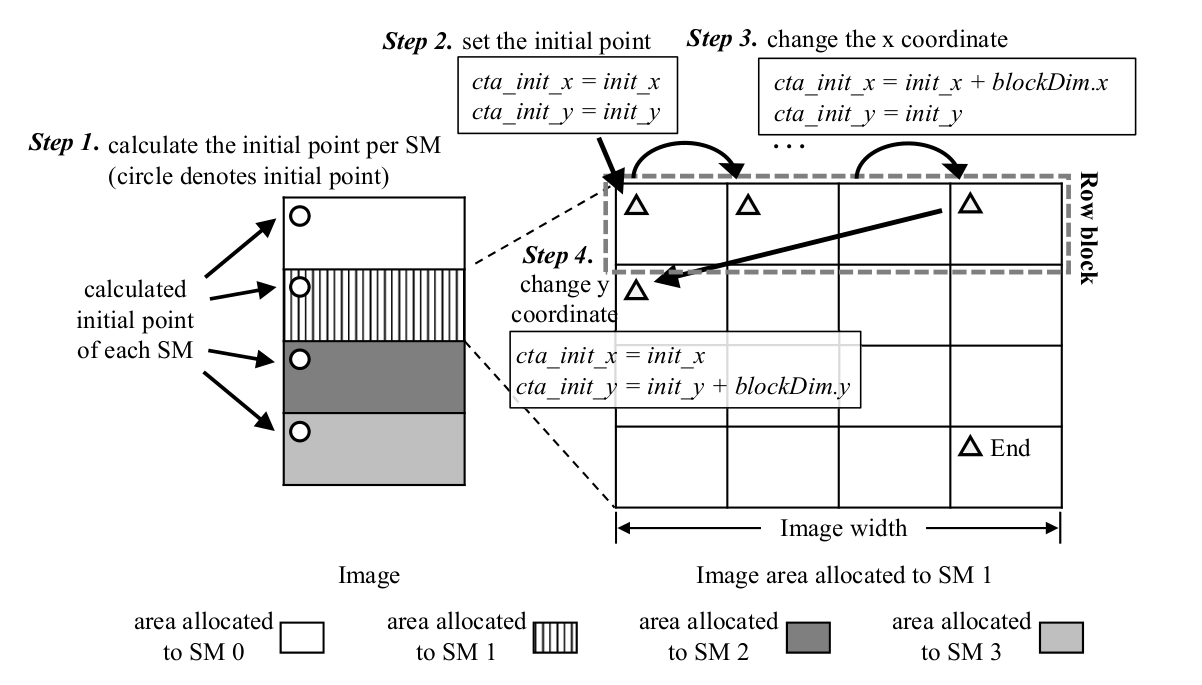
\includegraphics[width=0.9\textwidth]{Figure-1.png}
	\caption{Software-based row major pattern aware data allocation example.}
	\label{fig:row_major_pattern}
\end{figure}
First, the initial coordinate of the area allocated to each SM is calculated \textit{(Step 1)}. Then, the top-left coordinate for the first CTA execution denoted by a triangle is set to be the initial coordinate \textit{(Step 2)}. Following the CTA execution, the x-coordinate is moved in the row-major direction \textit{(Step 3)}. \textit{Step 3} is repeated until the execution is finished in the first row block, and then the process is moved to the next row block \textit{(Step 4)}. \textit{Steps 3} and \textit{Step 4} are repeated until the execution is finished for the entire data area allocated to SM0.\\

\textit{B. NDP GPU Architecture}\\
\textbf{SM Structure:} The number of warps and the size of on-chip SRAM that are appropriate for the SM structure of NDP GPU are proposed in this section.

\begin{enumerate}[label=(\arabic*)]
	\item Pattern-aware prefetcher: A stride-based prefetcher is mounted inside the SM of NDP GPU. Because the data access pattern of the algorithm is preserved through the proposed data allocation, accurate prefetching is provided with a simple stride-based prefetcher.
	\item The number of active warps: The access pattern-aware data allocation and prefetching make the necessary data readily available. Accordingly, as the stall decreases, the latency may be hidden with a smaller number of warps compared to the baseline GPU.
	\item On-chip SRAM size: The size of on-chip SRAM, including the register, L1 data cache, and shared memory, is reduced by using a smaller number of warps.
\end{enumerate}

\textbf{Off-chip L2 Cache:} The proposed NDP GPU uses no L2 cache. Data allocation and the prefetcher in the proposed NDP GPU help to increase the hit rate of the L1 cache to nearly 100\%, reducing the need for an L2 cache, which typically mitigates the miss penalty of the L1 cache in the memory hierarchy.

\textbf{The number of SMs:} Area constraints of the logic die should be considered along with performance and energy consumption to determine the optimal number of SMs for the NDP GPU.

\section{EVALUATION}

A cycle-accurate simulator, GPGPU-Sim \cite{ref4}, is modified to verify the impact of the proposed NDP architecture. Four configurations are evaluated as listed below.

\begin{itemize}
	\item Host: This is a conventional GPU. It is similar to the NVIDIA Maxwell GPU \cite{ref5} and has 64 SMs.
	\item B-NDP-L2: This denotes a baseline NDP with L2 cache. It has the same SM architecture as Host, but it is located on the logic die.
	\item B-NDP-woL2: This denotes a baseline NDP where the L2 cache is not used. Other configurations are the same as with B-NDP-L2.
	\item IP-NDP: This is the proposed NDP specialized for image processing. It has a prefetcher and a reduced-size SRAM.
\end{itemize}

Six commonly used image processing algorithms are tested \cite{ref6, ref7}. For the evaluation of IP-NDP, the code is modified according to the proposed method.

\begin{figure}[H]
	\centering
	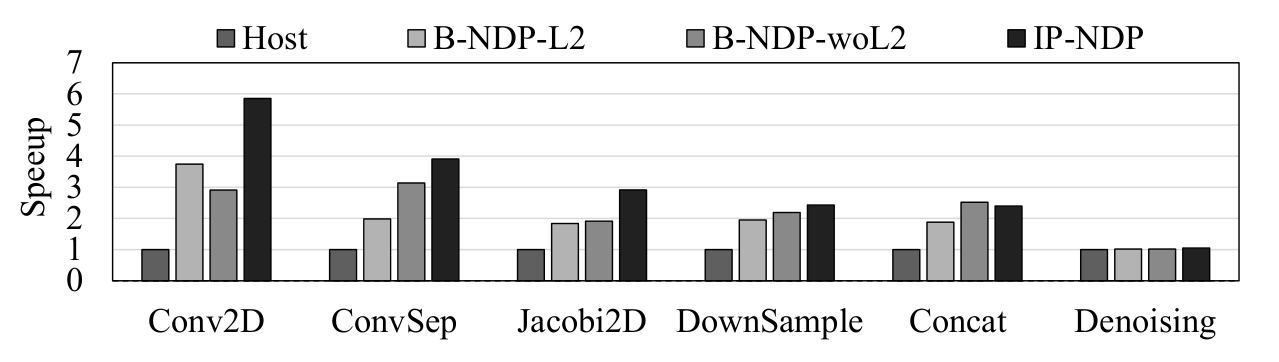
\includegraphics[width=\textwidth]{Figure-2.png}
	\caption{Speedup for B-NDP-L2, B-NDP-woL2, IP-NDP with varying the
		number of SMs in the NDP stack. All results are normalized to Host.}
	\label{fig:speedup_sms}
\end{figure}

Fig. 2 shows the increase in speed for the four configurations normalized to Host. Two observations from this result are explained below. First, image processing benefits from the increased bandwidth. B-NDP-L2 shows a 2.06× performance improvement on average over Host. Second, the proposed IP-NDP outperforms other configurations. IP-NDP is 3.09× (up to 5.85×), 1.44× (up to 1.97×), and 1.31× (up to 2.01×) faster than Host, B-NDP-L2, and B-NDP-woL2, respectively.

Thus, it can be concluded that the proposed pattern-aware data allocation and NDP GPU works very well. Although not shown in this paper, the proposed scheme consumes 52\% less energy than Host due to lower static power and faster execution, while requiring only 57.3\% of the area compared to Host.

\begin{center}
	ACKNOWLEDGMENT
\end{center}

This paper was the result of the research project supported by SK hynix Inc. and by the R\&D program of MOTIE/KEIT [No. 10077609, Developing Processor-Memory-Storage Integrated Architecture for Low Power, High Performance Big Data Servers]

\bibliographystyle{plain}
\bibliography{reference} 



\end{document}